\documentclass{beamer}
\usepackage{hyperref}
\usetheme{Madrid}
\usepackage{listings}
\usepackage{amsmath}
\usepackage{graphicx}
\usepackage{xcolor}
\definecolor{darkgreen}{rgb}{0.1, 0.5, 0.3}
\usepackage{fontawesome}

\title{Atomic Habits}
\author{James Clear}
\date{\today}

\begin{document}

\maketitle

\section{The Surprising Power of Atomic Habits}

\begin{frame}
    \frametitle{The Surprising Power of Atomic Habits}
    \begin{itemize}
        \item Change of fate of British Cyclists at 2003 : Dave Brailsford as new coach
        \item Not winning Tour de France for last 110 years
        \item \textcolor{darkgreen}{The aggregation of Marginal Gain} : philosophy of searching for a tiny margin of improvement in everything you do
        \begin{itemize}
            \item If you broke down everything you could think of that goes into riding a bike, and then improve it by 1 percent, you will get a significant increase when you put them all together
        \end{itemize}
    \end{itemize}
\end{frame}



\begin{frame}
    \frametitle{The Surprising Power of Atomic Habits}
    \begin{itemize}
        \item \textcolor{darkgreen}{small adjustments}:
        \begin{itemize}
            \item Redesigned the bike seats to make them more comfortable
            \item Rubbed alcohol on the tires for a better grip
            \item Electrically heated overshorts to maintain ideal muscle temperature while riding
            \item Biofeedback sensors to monitor how each athlete responded to a particular workout
            \item tested various fabrics in a wind tunnel and had their outdoor riders switch to indoor racing suits (lighter and aerodynamic)
            \item Painted the inside of the team truck white, which helped them spot little bits of dust that would normally slip by unnoticed but could degrade the performance of the finely tuned bikes.
        \end{itemize}
        \item British Cycling team \textcolor{orange}{dominated the road and track cycling} events after 5 years
        \item Five Tour de France victories in six years
    \end{itemize}
\end{frame}




\begin{frame}
    \frametitle{The Surprising Power of Atomic Habits}
    \textbf{WHY SMALL HABITS MAKE A BIG DIFFERENCE}
    \begin{itemize}
        \item Easy to overestimate the importance of one defining moment and underestimate the value of making small improvements on a daily basis
        \item Already convinced ourselves that massive success requires massive action
        \item We put \textcolor{darkgreen}{pressure} on ourselves to \textcolor{darkgreen}{make some earth-shattering improvement} that everyone will talk about for achieving any goal
        \item  \textcolor{orange}{Improving by 1 percent} can be far \textcolor{orange}{more meaningful}, especially in the long run.
    \end{itemize}
\end{frame}


\begin{frame}
    \frametitle{The Surprising Power of Atomic Habits}
    \textbf{1\% BETTER EVERY DAY}
    \begin{itemize}
        \item 1\% worse every day for one year. 0.99365 = 00.03
        \item 1\% better every day for one year. 1.01365 = 37.78
    \end{itemize}
    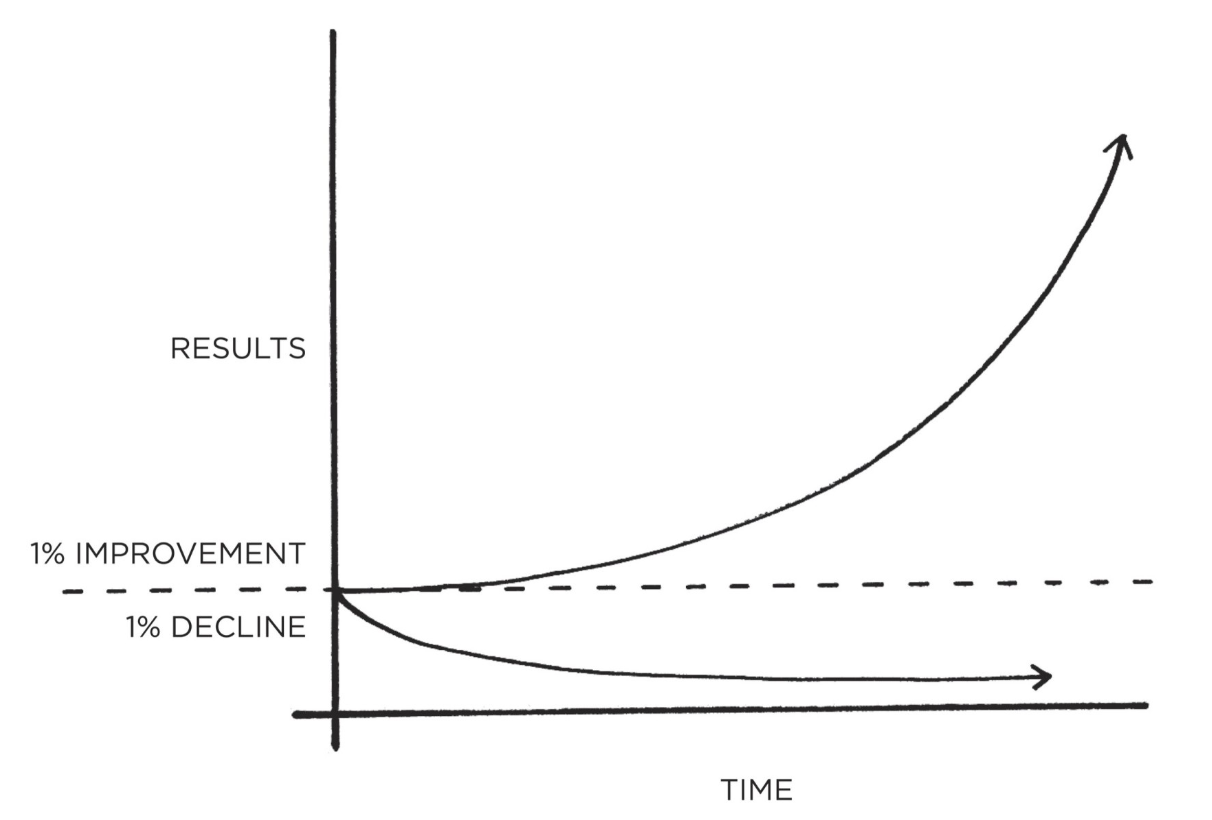
\includegraphics[width=4.0in, height=2.5in]{img1.png}\\
\end{frame}




\begin{frame}
    \frametitle{The Surprising Power of Atomic Habits}
    \begin{itemize}
        \item \textcolor{darkgreen}{Habits are the compound interest of selfimprovement}
        \item Above is a \textcolor{darkgreen}{difficult concept to appreciate} in daily life since small changes are being dismissed because they \textcolor{darkgreen}{seemingly doesn't matter very much in the moment}
        \begin{itemize}
            \item Saving a little money now, doesn't make you a millionaire 
            \item Studying Mandarin for an hour tonight doesn't make you Mandarin expert
        \end{itemize}
        \item Unfortunately, the \textcolor{red}{slow pace of transformation} also makes it easy to \textcolor{red}{let a bad habit slide}
        \begin{itemize}
            \item eat an unhealthy meal today : \textcolor{gray}{ the scale doesn’t move much}
            \item work late tonight and ignore your family : \textcolor{gray}{they will forgive you}
            \item procrastinate and put your project off until tomorrow : \textcolor{gray}{there will usually be time to finish it later}
        \end{itemize}
        \item A single decision is easy to dismiss.
        
    \end{itemize}
\end{frame}




\begin{frame}
    \frametitle{The Surprising Power of Atomic Habits}
    \begin{itemize}
        \item when we \textcolor{darkgreen}{repeat 1 percent errors, day after day}
        \begin{itemize}
            \item  by replicating poor decisions
            \item  duplicating tiny mistakes
            \item rationalizing little excuses
        \end{itemize}our \textcolor{darkgreen}{small choices} \textcolor{red}{compound} into \textcolor{red}{toxic results}
        \item \textcolor{darkgreen}{Impact} created by a \textcolor{darkgreen}{change in your habits} is similar to the \textcolor{darkgreen}{effect of shifting the route of an airplane} by \textcolor{darkgreen}{just a few degrees}
        \item a \textcolor{darkgreen}{slight change} in your \textcolor{darkgreen}{daily habits} can guide your life to a \textcolor{orange}{very different destination}
    \end{itemize}
    \begin{center}
    {\large \textit{“Success is the product of daily habits—not once-in-a-lifetime transformations”}}  
    \end{center}
    
\end{frame}


\begin{frame}
    \frametitle{The Surprising Power of Atomic Habits}
\end{frame}

\end{document}